	For the use of infrared thermography it can be found studies for inspection application. The infrared camera makes possible to work with thermal information in entire areas covered by the field of view, different from thermocouples that are able to measure punctual temperatures for example.

	\citeonline{lee2011study} shows a study on integrity of resistance spot welding by means of infrared thermography. It was set two external heat sources in order to raise the temperature of the spot. The results have shown a promising method of inspection when comes to diameter measurement of the nugget. While measurements made with naked eye provide a difference of about 20\%, the thermography provides only 8\%.

	Also \citeonline{lebar2010method} developed a method that allows online thermal measurement of abrasive water jet cutting. The method makes possible to extract features of thermal image and to correlate with texture analysis of the workpiece afterwards. This is important to evaluate the cutting process performance.

	\begin{figure}[H]
		\centering
		\captionsetup{justification=centering}
		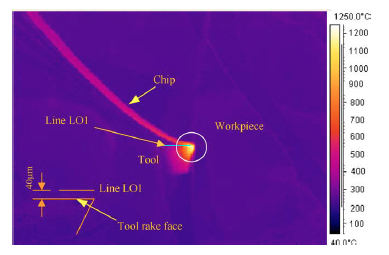
\includegraphics[scale=0.75]{Cap2/InfraRed/exinfrared.png}
		\caption{Infrared photography of a cutting process \cite{abukhshim2006heat}}
		\label{fig:exinfrared}
	\end{figure}

	For the case under study, high speed thermography has its positive and negative points. On the positive side, it may be mentioned:

	\begin{itemize}
		\item Fast inspection rate (reasonable number of images of high speed cutting)
		\item Contactless (no interference during the cutting process)
		\item Easy interpretation of the results (indexed image with temperatures in each pixel)
	\end{itemize}

	But it is also important to mention the difficulties that in this method still prevail:
	
	\begin{itemize}
		\item Only a limited thickness can be measured (under the main surface)
		\item Determine a suitable emissivity is a chalenge (it changes with temperature variation)
	\end{itemize}
